\chapter{Methods}

This chapter will detail the methods employed in this thesis to integrate SCVAEs and non-conditioned VAEs using multitask learning, focusing specifically on image data. For clarity, the chapter will be divided into four sections.

The initial section will describe the various conditioning strategies that were employed in this thesis. Following this, the subsequent section will delve into the methodology of combining SCVAEs with non-conditioned VAEs utilizing dual decoders - one conditioned and the other unconditioned. This method will be referred to as \methodOne{1}. Subsequently, another method of merging SCVAEs with non-conditioned VAEs will be presented in the subsequent section. This approach involves utilizing a single decoder for both tasks by employing novel training strategies, which will be referred to as \methodTwo{2}. It is important to note that both methods will be applied to both Gaussian VAEs and VQ-VAEs.

The final section outlines the experimental setup that was used to evaluate the proposed methods, whilst also providing a brief overview of the datasets, network architecture, and hyperparameters used in the experiments.

\section{Conditioning information}

In this thesis, I will obtain the conditioning information $m$ from the input
image $x$ by sampling some pixels from the input image $x$. In this
process, the first step is to obtain a mask which will be used to sample
the pixels from the input image $x$. The mask will be a binary matrix of the
same size as the input image $x$, where a value of 1 represents the sampled
pixels and a value of 0 represents the pixels that are not sampled. The
decision of how many pixels to sample and which pixels to sample will be described
in the following sections for each method.

After the mask is obtained, the mask is applied to the input image $x$ to
obtain the masked image, which is then used to obtain the conditioning
information $m$ by concatenating the mask with the masked image, which can be
seen in Figure~\ref{ConditioningFigure}.

In both proposed methods, the conditioning information $m$ will be incorporated
into the decoder by first flattening it and then concatenating it with the input of the decoder and then using a fully connected layer before passing it through the transposed convolutional layers of the decoder.

\begin{figure}
    \centering
    \tikzset{every picture/.style={line width=0.75pt}} %set default line width to 0.75pt        

\begin{tikzpicture}[x=0.75pt,y=0.75pt,yscale=-1,xscale=1]
%uncomment if require: \path (0,300); %set diagram left start at 0, and has height of 300

%Image [id:dp8071272108239995] 
\draw (189,81.67) node  {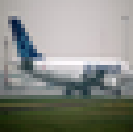
\includegraphics[width=52.5pt,height=52.5pt]{figures/assets/ORIGINAL_GAUSSIAN.png}};
%Image [id:dp988855448482646] 
\draw (188.33,176) node  {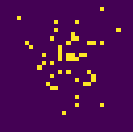
\includegraphics[width=52.5pt,height=52.5pt]{figures/assets/MASK_GAUSSIAN.png}};
%Image [id:dp22673392822113958] 
\draw (309.67,103.67) node  {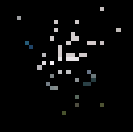
\includegraphics[width=52.5pt,height=52.5pt]{figures/assets/RESULT_GAUSSIAN.png}};
%Curve Lines [id:da7064061111049843] 
\draw    (224.33,86.33) .. controls (257.99,82.37) and (227.62,107.16) .. (272.29,100.54) ;
\draw [shift={(273.67,100.33)}, rotate = 171.07] [color={rgb, 255:red, 0; green, 0; blue, 0 }  ][line width=0.75]    (10.93,-3.29) .. controls (6.95,-1.4) and (3.31,-0.3) .. (0,0) .. controls (3.31,0.3) and (6.95,1.4) .. (10.93,3.29)   ;
%Curve Lines [id:da2412457613293979] 
\draw    (224.33,157.67) .. controls (273.83,153.05) and (228.59,124.9) .. (272.96,117.23) ;
\draw [shift={(274.33,117)}, rotate = 171.07] [color={rgb, 255:red, 0; green, 0; blue, 0 }  ][line width=0.75]    (10.93,-3.29) .. controls (6.95,-1.4) and (3.31,-0.3) .. (0,0) .. controls (3.31,0.3) and (6.95,1.4) .. (10.93,3.29)   ;
%Image [id:dp7901210362437346] 
\draw (431,111.33) node  {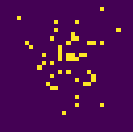
\includegraphics[width=52.5pt,height=52.5pt]{figures/assets/GREEN_GAUSSIAN.png}};
%Image [id:dp9948313666469564] 
\draw (423.67,123) node  {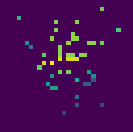
\includegraphics[width=52.5pt,height=52.5pt]{figures/assets/RED_GAUSSIAN.png}};
%Shape: Square [id:dp655934035728707] 
\draw  [color={rgb, 255:red, 255; green, 255; blue, 255 }  ,draw opacity=1 ] (388.67,88) -- (458.67,88) -- (458.67,158) -- (388.67,158) -- cycle ;
%Image [id:dp29091288526835224] 
\draw (417,136) node  {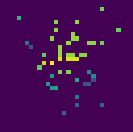
\includegraphics[width=52.5pt,height=52.5pt]{figures/assets/BLUE_GAUSSIAN.png}};
%Shape: Square [id:dp17919766367981604] 
\draw  [color={rgb, 255:red, 255; green, 255; blue, 255 }  ,draw opacity=1 ] (382,101) -- (452,101) -- (452,171) -- (382,171) -- cycle ;
%Image [id:dp6261788477655241] 
\draw (411,148.67) node  {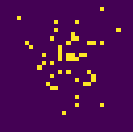
\includegraphics[width=52.5pt,height=52.5pt]{figures/assets/MASK_GAUSSIAN.png}};
%Shape: Square [id:dp8527153376534193] 
\draw  [color={rgb, 255:red, 255; green, 255; blue, 255 }  ,draw opacity=1 ] (376,113.67) -- (446,113.67) -- (446,183.67) -- (376,183.67) -- cycle ;
%Curve Lines [id:da0011889641265926398] 
\draw    (345.67,104.33) .. controls (353.15,122.41) and (361.21,123.58) .. (369.86,125.84) ;
\draw [shift={(371.67,126.33)}, rotate = 195.95] [color={rgb, 255:red, 0; green, 0; blue, 0 }  ][line width=0.75]    (10.93,-3.29) .. controls (6.95,-1.4) and (3.31,-0.3) .. (0,0) .. controls (3.31,0.3) and (6.95,1.4) .. (10.93,3.29)   ;
%Curve Lines [id:da5210657288496086] 
\draw    (224.33,169.67) .. controls (267.89,153.83) and (323.87,157.59) .. (372.2,149.26) ;
\draw [shift={(373.67,149)}, rotate = 169.9] [color={rgb, 255:red, 0; green, 0; blue, 0 }  ][line width=0.75]    (10.93,-3.29) .. controls (6.95,-1.4) and (3.31,-0.3) .. (0,0) .. controls (3.31,0.3) and (6.95,1.4) .. (10.93,3.29)   ;

% Text Node
\draw (162,27.33) node [anchor=north west][inner sep=0.75pt]   [align=left] {Original};
% Text Node
\draw (168.67,123.33) node [anchor=north west][inner sep=0.75pt]   [align=left] {Mask};
% Text Node
\draw (420.67,50.67) node [anchor=north west][inner sep=0.75pt]   [align=left] {$\displaystyle m$};


\end{tikzpicture}

    \caption[The illustration of the process of obtaining the conditioning information $m$ from the input image $x$ and the mask.]%
    {
        The illustration of the process of obtaining the conditioning information $m$ from the input image $x$ and the mask. The process to obtain the conditioning information $m$ consists of two steps: the first step is to obtain the masked image from the input image $x$ and the mask, and the second step is to add the mask to the masked image to obtain the conditioning information $m$. The conditioning information $m$ is then used to condition the decoder.
    }\label{ConditioningFigure}
\end{figure}

\section{\methodOne{1}}

In the first method, the VAE framework is expanded with a second decoder
$p_\xi(x|z,m)$, which is conditioned on an additional property $m$ of the input
data. This approach involves utilizing two decoders within the VAE framework:
one for reconstructing the input data solely based on a trained neural network with \methodOne{1} latent variable $z$,
and the other for reconstructing the input data based on both the latent
variable $z$ and the additional conditioning information $m$, see Figures \ref{SCVAE2DFigure} and \ref{SCVQVAE2DFigure}.

\subsection{Conditioning strategy}

In this method, the conditioning information $m$ is acquired by sampling a
constant number of pixels from the input data. To sample the pixels from the
input image $x$, I will use a pixel sampling operation, which will be described
in the following section.

\subsubsection{Pixel Sampling operation}

I will explore two-pixel sampling types for this method,
which can be seen in Figure~\ref{SamplingFigure} and are described as follows:

\begin{enumerate}
    \item \textbf{Exact Sampling:} In this sampling type, the conditioning information $m$ is sampled from the input image $x$ by sampling the same sparse pixels from the input image $x$. In this work, the pixels that will be sampled from the input image will be a sparse grid of pixels.
    \item \textbf{Uniform Random Sampling:} In this sampling type, the conditioning information $m$ is sampled from the input image $x$ by sampling the exact number of pixels from the input image $x$ uniformly at random.
\end{enumerate}

The sampling process will be done every time the input image $x$ is passed through the model. This means that in the case of the Uniform Random Sampling, the conditioning information $m$ will be different for each time the image is passed through the model. This is done to ensure that the model learns to generalize and handle various cases.

\subsection{Application to Gaussian VAEs}

In Gaussian VAEs, the integration of a second conditioned decoder
$p_\xi(x|z,m)$ follows a similar approach as outlined in the general method
description. However, some specific adjustments and considerations need to be taken into account when applying this method to Gaussian VAEs.

The integration of the second conditioned decoder $p_\xi(x|z,m)$ into the
Gaussian VAEs framework involves flattening and concatenating the latent
variable $z$ and the conditioning information $m$ and passing it through a
fully connected layer before passing it through the transposed convolutional
layers of the second decoder. Although a new latent variable could have
been sampled for the second decoder, the same latent variable $z$ is used
instead of sampling a new one. This is done to ensure that the latent variable
$z$ is the same for both decoders and ensures that it is easier to compare the
reconstructions of the input data. The architecture of the Gaussian
VAE framework with the second conditioned decoder is illustrated in
Figure~\ref{SCVAE2DFigure}

Although the training strategy could have been to train decoders by alternating between them, in this thesis, I will explore the training strategy where both decoders are trained simultaneously.

In Gaussian VAEs, the loss objective consists of two components: the
reconstruction loss and the KL divergence term. However, with the inclusion of
the second conditioned decoder, the loss objective is extended to include the
reconstruction loss of the second conditioned decoder. The overall loss
objective to be \textbf{minimized} becomes

\[ L = W_1 \frac{1}{D} \sum_{i=1}^{D} ||x_i - \hat{x}_{1_{i}} ||^2 + W_2 \frac{1}{D} \sum_{i=1}^{D} || x_i - \hat{x}_{2_{i}} ||^2 + \beta  \frac{1}{2} \sum_{i=1}^{Z} \biggl( -\log \sigma^2_\phi(x)_i - 1 + \mu^2_\phi(x)_i + \sigma^2_\phi(x)_i \biggr), \]

where $D$ is the number of pixels in the input image, $x_i$ is the $i$-th pixel
of the input image, $\hat{x}_1$ is the output of the first decoder, $\hat{x}_2$
is the output of the second decoder, $\beta$ is the KL divergence weight, Z is
the dimension of the latent space, $\mu_\phi(x)$ and $\sigma_\phi(x)$ are the
mean and the standard deviation of the Gaussian distribution produced by the
encoder, respectively. The resulting loss has also extra weight parameters $W_1$ and $W_2$ to balance and control the importance of reconstruction loss, which will be hyperparameters of the model.

During the training process, the encoder is trained to produce an accurate mean
and standard deviation of the Gaussian distribution, and the decoders are
trained to produce accurate reconstructions of the input data.

As a result of the integration of the second conditioned decoder, the model has
the ability to reconstruct the input data based just on the latent variable $z$
and as well as the conditioning information $m$.
\begin{figure}[H]
    \centering
    \centering
\scriptsize
\begin{tabular}{||c|c|c|c||}
\hline
 Method & Parameters & Reconstruction loss & KL loss \\
\hline
\textit{Baseline} & - & 0.0042 +- 1.2e-03 & 0.0018 +- 6.3e-04 \\
\hline
Multi Decoder & Exact sampling & 0.0036 +- 8.3e-04  $\downarrow$ & 0.0027 +- 8.7e-04  $\uparrow$ \\
\hline
Multi Decoder & Exact sampling, SoftAdapt & 0.0034 +- 1.9e-04  $\downarrow$ & 0.0029 +- 2.8e-03  $\uparrow$ \\
\hline
Multi Decoder & Uniform sampling & 0.0035 +- 6.5e-04  $\downarrow$ & 0.0026 +- 1.7e-03  $\uparrow$ \\
\hline
Multi Decoder & Uniform sampling, SoftAdapt & 0.0034 +- 7.3e-03  $\downarrow$ & 0.0029 +- 2.0e-02  $\uparrow$ \\
\hline
\end{tabular}

    \caption[\methodOne{1} applied to Gaussian VAEs.]%
    {
        \methodOne{1} applied to Gaussian VAEs. The Gaussian VAEs framework is extended by adding a second conditioned decoder $p_\xi(x|z,m)$. The input $x$ is passed through the encoder with parameters $\phi$ producing the mean $\mu$ and the standard deviation $\sigma$ of the Gaussian distribution. The random variable $\epsilon$ is sampled from a standard Gaussian distribution and is used to sample $ z = \mu + \sigma \odot \epsilon$. The sampled $z$ is then used as input to both decoders. As a result, the loss function consists of three components: the MSE reconstruction loss of the first decoder, the MSE reconstruction loss of the second decoder and the KL divergence regularization loss.
    }\label{SCVAE2DFigure}
\end{figure}

\subsection{Application to VQ-VAEs}

The approach of integrating the second conditioned decoder $p_\xi(x|z,m)$ into
the VQ-VAEs framework is similar to the approach used for Gaussian VAEs.
However, some differences need to be taken into account when applying
this method to VQ-VAEs.

One of the main differences is that the VQ-VAEs framework uses a discrete
latent space and the Vector Quantization which is described in \autoref{background:vqvae}. This means that the latent variable $z$ is a discrete variable that represents the indexes of the embedding table vectors. This means that first the corresponding embedding table vectors $z_q(x)$ must be computed for the latent variable $z$ before flattening and concatenating it with the conditioning information $m$ and then using a fully connected layer before the transposed convolutional layers of the second decoder. The architecture of the VQ-VAEs framework with the second conditioned decoder is illustrated in Figure~\ref{SCVQVAE2DFigure}.

The training strategy is the same as in Gaussian VAEs, where both decoders are trained simultaneously. This means that the loss objective must be extended to include the reconstruction loss of the second conditioned decoder. In VQ-VAEs, the loss objective consists of three components: the MSE reconstruction loss, the commitment loss and the codebook loss. However, with the inclusion of the second conditioned decoder, the loss objective is
extended to include the reconstruction loss of the second conditioned decoder.
The overall loss objective to be \textbf{minimized} becomes

\[ L = W_1 \frac{1}{D} \sum_{i=1}^{D} ||x_i - \hat{x}_{1_{i}} ||^2 +  W_2 \frac{1}{D} \sum_{i=1}^{D} || x_i - \hat{x}_{2_{i}} ||^2 + \frac{1}{Z} \sum_{i=1}^{Z} \biggl( || sg(z_e(x)_i) - e_{k_i} ||^2 + \beta || z_q(x)_i - sg(e_{k{_i}}) ||^2 \biggr) , \]

% TODO explain the weights W1 and W2

where $D$ is the number of pixels in the input image, $x_i$ is the $i$-th pixel
of the input image, $\hat{x}_1$ is the output of the first decoder, $\hat{x}_2$
is the output of the second decoder, $Z$ is the number of latent space vectors,
$z_e(x)$ is the output of the encoder, $z_q(x)$ is the mapping output after
Vector Quantization, $e_k$ is the $k$-th embedding table vector, $\beta$ is the
commitment loss weight, $sg$ is the stop gradient operation, which was
previously defined in the background \autoref{background:vqvae}.

After the first stage of the training, the model has the ability to reconstruct
the input data based just on the latent variable $z$ and as well as the
conditioning information $m$. To generate the latent variable $z$, one must
train a separate autoregressive model, which will be used to generate the
latent variable $z$.

\begin{figure}[H]
    \centering
    \centering
\scriptsize
\begin{tabular}{||c|c|c|c||}
\hline
 Method & Parameters & Reconstruction loss & VQ loss \\
\hline
\textit{Baseline} & - & 0.0022 +- 7.4e-08 & 0.0029 +- 4.1e-07 \\
\hline
Multi Decoder & Exact sampling & 0.0017 +- 6.9e-09  $\downarrow$ & 0.0039 +- 9.8e-07  $\uparrow$ \\
\hline
Multi Decoder & Exact sampling, SoftAdapt & \textbf{0.0013 +- 2.4e-09}  $\downarrow$ & \textbf{0.0016 +- 6.8e-08}  $\downarrow$ \\
\hline
Multi Decoder & Uniform sampling & 0.0018 +- 1.3e-07  $\downarrow$ & 0.0036 +- 3.5e-07  $\uparrow$ \\
\hline
Multi Decoder & Uniform sampling, SoftAdapt & \textbf{0.0017 +- 6.6e-08}  $\downarrow$ & \textbf{0.0021 +- 3.1e-07}  $\downarrow$ \\
\hline
\end{tabular}

    \caption[\methodOne{1} applied to VQ-VAEs.]%
    {
        \methodOne{1} applied to VQ-VAEs. The VQ-VAEs framework is extended by adding a second conditioned decoder. Instead of using a fully connected layer to merge the latent variable $z$ and the conditioning information $m$, the corresponding embedding table vectors $z_q(x)$ must be computed for the latent variable $z$ before merging it with the conditioning information $m$. As a result of adding the second conditioned decoder, the loss function requires the addition of the MSE reconstruction loss of the second decoder.
    }\label{SCVQVAE2DFigure}
\end{figure}

\section{\methodTwo{2}}

In the \methodTwo{2}, the idea is to employ a single decoder within the VAE architecture that is capable of reconstructing the input data under variable conditioning. Variable conditioning means that the conditioning information $m$ can be a variable amount of information or just an empty mask. This method differs from the \methodOne{1} in that it uses a single decoder for both tasks and dynamically adjusts its behavior based on the amount of information present in the variable $m$.

This method utilizes a single decoder that dynamically adjusts its behavior
based on the amount of information present in the variable $m$. When the
conditioning information is available, the decoder incorporates it into the
reconstruction process and takes advantage of it to get the best
reconstruction. Otherwise, it operates solely based on the latent variable $z$.

To achieve this, in this method, I will use different conditioning strategies, which will be described in the following subsection.

\subsection{Conditioning strategy}

Similar to the previous method, the conditioning information $m$ is acquired by
sampling pixels from the input image $x$. However, in this method, the process of sampling the conditioning information $m$ is different in that the conditioning information $m$ is sampled by selecting a variable number of pixels from the input image $x$. This is done to ensure that the decoder of the model learns to handle various cases where there is variable conditioning information.

To achieve this, I will implement a two-step sampling process:

\begin{enumerate}
    \item \textbf{Sampling the number of pixels:} In this step, the number of pixels to be sampled from the input image $x$ is sampled from a power law distribution. The power law distribution is scaled to the size of the input image $x$ and is used to sample the number of pixels to be sampled from the input image $x$.
    \item \textbf{Sampling the pixels:} In this step, the conditioning information $m$ is sampled from the input image $x$ by sampling the number of pixels sampled in the previous step from the input image: uniformly at random or from a Gaussian distribution. Both of these sampling types can be seen in Figure~\ref{SamplingFigure}.
\end{enumerate}

The sampling two-step process will be done every time the input image $x$ is passed through the model. This means that the conditioning information $m$ will be different for each time the image is passed through the model. This is done to ensure that the model learns to generalize and handle various cases.

During training, the number of pixels to be sampled from the input image $x$ varies every time the input image $x$ is passed through the model and is sampled from a power law distribution.
The power law distribution is chosen because it can have a finite range and scalability, which makes it suitable for sampling the number of pixels from the input image. The exponent of the power law distribution will be chosen to be high so that the decoder can learn to handle also the cases where the conditioning information is not available. The exponent will be a hyperparameter of the model.


\subsection{Application to Gaussian VAEs}

In Gaussian VAEs, applying the second method involves modifying the decoder to
be capable of reconstructing the input data under variable conditioning. The
modified decoder $p_\xi(x|z,m)$ is capable of reconstructing the input data
based on the latent variable $z$ and the conditioning information $m$ or just
the latent variable $z$ if the conditioning information is not available and is just an empty mask filled with zeros.

This is achieved by using a fully connected layer to merge the latent variable
$z$ and the conditioning information $m$ before passing it through the
transposed convolutional layers. The architecture of the Gaussian VAEs
framework with a single decoder capable of variable conditioning is illustrated
in Figure~\ref{SCVAE1DFigure}.

\begin{figure}[H]
    \centering
    \centering
\scriptsize
\begin{tabular}{||c|c|c|c||}
\hline
 Method & Parameters & Reconstruction loss & KL loss \\
\hline
\textit{Baseline} & - & 0.0097 +- 4.2e-03 & 63.0518 +- 2.4e+01 \\
\hline
Single Decoder & Gaussian sampling, Exponent=40 & 0.0113 +- 1.4e-02  $\uparrow$ & 54.7483 +- 7.3e+01  $\downarrow$ \\
\hline
Single Decoder & Gaussian sampling, Exponent=60 & 0.0113 +- 2.6e-03  $\uparrow$ & 54.6946 +- 4.4e+01  $\downarrow$ \\
\hline
\end{tabular}

    \caption[\methodTwo{2} applied to Gaussian VAEs.]%
    {
        \methodTwo{2} applied to Gaussian VAEs. The Gaussian VAEs framework is modified by allowing the decoder to be conditioned on a variable amount of information and to dynamically adjust its behavior based on the amount of information present in the variable $m$. The input $x$ is passed through the encoder with parameters $\phi$ producing the mean $\mu$ and the standard deviation $\sigma$ of the Gaussian distribution. The random variable $\epsilon$ is sampled from a standard Gaussian distribution and is used to sample $ z = \mu + \sigma \odot \epsilon$. The sampled $z$ is then used as input to the decoder as well as the extra conditioning information $m$. With this approach, there is no need for a second decoder, as the single decoder is capable of reconstructing the data based on the latent variable $z$ and the conditioning information $m$ or just the latent variable $z$.
    }\label{SCVAE1DFigure}
\end{figure}

\subsection{Application to VQ-VAEs}

In VQVAEs, the same as in Gaussian VAEs, the second method involves modifying the
decoder to be capable of receiving variable conditioning information. Unlike
Gaussian VAEs, the VQ-VAEs use Vector Quantization to discretize the continuous 
latent space, which is described in \autoref{background:vqvae}. Since the latent
variable $z$ is just a representation of the indexes of the embedding table vectors, the latent variable $z$ must be first mapped to the corresponding embedding table vectors resulting in $z_q(x)$ representation. Then the same process as in Gaussian VAEs is applied where the latent variable $z_q(x)$ and the conditioning information $m$ are merged using a fully connected layer before passing it through the transposed convolutional layers of the decoder. The architecture of the VQ-VAEs framework with a single decoder capable of
variable conditioning is illustrated in Figure~\ref{SCVQVAE1DFigure}.

\begin{figure}[H]
    \centering
    \centering
\scriptsize
\begin{tabular}{||c|c|c|c||}
\hline
 Method & Parameters & Reconstruction loss & VQ loss \\
\hline
\textit{Baseline} & - & 0.0022 +- 4.2e-08 & 0.0048 +- 8.3e-07 \\
\hline
Single Decoder & Gaussian sampling, Exponent=40 & 0.0026 +- 1.9e-07  $\uparrow$ & 0.0028 +- 2.3e-06  $\downarrow$ \\
\hline
Single Decoder & Gaussian sampling, Exponent=40 & 0.0023 +- 3.9e-07  $\uparrow$ & 0.0015 +- 7.3e-08  $\downarrow$ \\
\hline
Single Decoder & Gaussian sampling, Exponent=60 & 0.0029 +- 4.5e-07  $\uparrow$ & 0.0041 +- 4.1e-06  $\downarrow$ \\
\hline
Single Decoder & Gaussian sampling, Exponent=60 & \textbf{0.0020 +- 9.2e-08}  $\downarrow$ & \textbf{0.0013 +- 7.6e-08}  $\downarrow$ \\
\hline
Single Decoder & Uniform sampling, Exponent=40 & \textbf{0.0022 +- 1.1e-08}  $\downarrow$ & \textbf{0.0020 +- 2.2e-08}  $\downarrow$ \\
\hline
Single Decoder & Uniform sampling, Exponent=40 & \textbf{0.0022 +- 1.2e-07}  $\downarrow$ & \textbf{0.0018 +- 1.1e-08}  $\downarrow$ \\
\hline
Single Decoder & Uniform sampling, Exponent=60 & 0.0026 +- 7.2e-08  $\uparrow$ & 0.0030 +- 8.0e-07  $\downarrow$ \\
\hline
Single Decoder & Uniform sampling, Exponent=60 & 0.0023 +- 2.1e-07  $\uparrow$ & 0.0015 +- 9.0e-08  $\downarrow$ \\
\hline
\end{tabular}

    \caption[\methodTwo{2} applied to VQ-VAEs.]%
    {
        \methodTwo\ applied to VQ-VAEs. The VQ-VAEs framework is modified by allowing the decoder to be conditioned on a variable amount of information and to dynamically adjust its behavior based on the amount of information present in the variable $m$. The input $x$ is passed through the encoder producing the output $z_e(x)$. The output $z_e(x)$ is then used as input to the autoregressive model to generate the latent variable $z$. The latent variable $z$ is then used as input to the decoder as well as the extra conditioning information $m$. With this approach, there is no need for a second decoder, as the single decoder is capable of reconstructing the data based on the latent variable $z$ and the conditioning information $m$ or just the latent variable $z$.
    }\label{SCVQVAE1DFigure}
\end{figure}

\begin{figure}
    \centering
    

\tikzset{every picture/.style={line width=0.75pt}} %set default line width to 0.75pt        

\begin{tikzpicture}[x=0.75pt,y=0.75pt,yscale=-1,xscale=1]
%uncomment if require: \path (0,374); %set diagram left start at 0, and has height of 374

%Image [id:dp9293884018723756] 
\draw (365.67,295.2) node  {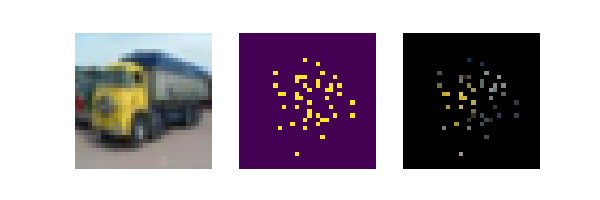
\includegraphics[width=225pt,height=75pt]{figures/assets/GAUSSIAN.png}};
%Image [id:dp548757972749888] 
\draw (365.67,208.8) node  {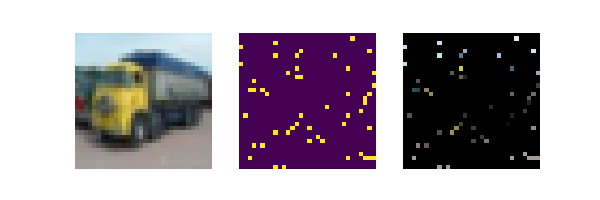
\includegraphics[width=225pt,height=75pt]{figures/assets/UNIFORM.png}};
%Image [id:dp620494998311241] 
\draw (365.67,124.8) node  {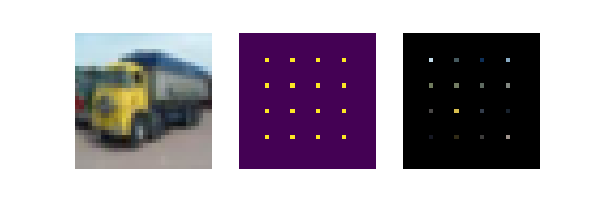
\includegraphics[width=225pt,height=75pt]{figures/assets/EXACT.png}};
%Shape: Grid [id:dp3074430629490833] 
\draw  [draw opacity=0] (242.67,82.33) -- (497.67,82.33) -- (497.67,337.67) -- (242.67,337.67) -- cycle ; \draw   (242.67,82.33) -- (242.67,337.67)(327.67,82.33) -- (327.67,337.67)(412.67,82.33) -- (412.67,337.67)(497.67,82.33) -- (497.67,337.67) ; \draw   (242.67,82.33) -- (497.67,82.33)(242.67,167.33) -- (497.67,167.33)(242.67,252.33) -- (497.67,252.33)(242.67,337.33) -- (497.67,337.33) ; \draw    ;

% Text Node
\draw (279.26,61.29) node [anchor=north west][inner sep=0.75pt]  [rotate=-308.3] [align=left] {original};
% Text Node
\draw (172.67,120) node [anchor=north west][inner sep=0.75pt]   [align=left] {Exact};
% Text Node
\draw (359.26,61.29) node [anchor=north west][inner sep=0.75pt]  [rotate=-308.3] [align=left] {original};
% Text Node
\draw (437.53,61.29) node [anchor=north west][inner sep=0.75pt]  [rotate=-308.3] [align=left] {original};
% Text Node
\draw (165.17,204) node [anchor=north west][inner sep=0.75pt]   [align=left] {Uniform};
% Text Node
\draw (160.17,291) node [anchor=north west][inner sep=0.75pt]   [align=left] {Gaussian};


\end{tikzpicture}

    \caption[Table of pixel sampling types for conditioning.]%
    {
        Table of pixel sampling types for conditioning. The table has 3 rows each representing a different sampling type. The first row represents the Exact Sampling type, the second row represents the uniform random sampling type and the third row represents the Gaussian sampling type where the pixels are more likely to be sampled from the center of the image. The first column represents the original image, the second column represents the mask and the third column represents the result of the sampling operation.
    }\label{SamplingFigure}
\end{figure}

\section{Experimental setup}

In this section, I will describe the experimental setup that was used to evaluate the proposed methods. The full code for experiments was implemented in Python using Pytorch library and is available on GitHub\footnote{\url{https://github.com/EdvardsZ/MastersThesis}}.

\subsection{Datasets}

The proposed methods were evaluated on the MNIST, CIFAR-10 and CelebA datasets. The MNIST dataset consists of 60,000 images of the size 28x28 pixels with 10 classes. The CIFAR-10 dataset consists of 60,000 colored images of the size 32x32 pixels with 10 classes.
The CelebA dataset consists of 202,599 images of celebrities with 10,177 identities and 40 binary attributes. In these experiments, the CelebA dataset images were resized to 64x64 pixels to reduce the computational complexity.
The datasets will be split into training, validation and test sets, where the training set will be used to train the models and the validation set will be used to evaluate.

\subsection{Network architecture and hyperparameters}

The encoder and the decoder of the models will be convolutional neural networks. The number of layers and the number of filters in each layer will be hyperparameters of the model. Both the encoder and the decoder will have a similar architecture of convolutional layers followed by batch normalization layers and LeakyReLU activation functions. However, the encoder and the decoder for the Gaussian VAEs will be more shallow compared to the VQ-VAEs, because the Gaussian VAEs suffer from the posterior collapse if the neural network is too deep. 

For Gaussian VAEs experiments were conducted in 2 configurations:

\begin{itemize}
    \item Config. 1: latent space dimension of 16, with hidden dimensions of 32, 64, 128, 256
    \item Config. 2: latent space dimension of 64, with hidden dimensions of 32, 64, 128, 256
\end{itemize}

For VQ-VAEs experiments were conducted in 3 configurations:

\begin{itemize}
    \item Config. 1: 128 embeddings and 16 the embedding dimension, hidden dimensions for both encoder and decoder were set to 32 and 64 and 0 residual layers.
    \item Config. 2: 128 embeddings and 32 the embedding dimension, hidden dimensions for both encoder and decoder were set to 128 and 256 and 2 residual layers.
    \item Config. 3: 256 embeddings and 64 the embedding dimension, hidden dimensions for both encoder and decoder were set to 128 and 256 and 4 residual layers.
\end{itemize}

\subsection{Training}

The models were trained using the AdamW optimizer with a learning rate of $10^{-3}$ and a batch size of 128 for 100 epochs. The best models were selected based on the cross-validation results. The models were trained on a single GPU.